
\chapter{背景分析}

排课,即课程编排,是指学校为了正常进行教学工作,对班级、教师、课程及学校教学资源合理安排,制定各种各样课程表的行为。%
给大学合理编排课程,不仅需要考虑课程之间的依赖关系:有些课程需要比其他课程更先修读;还要解决课程编排的合理性:不能一次性%
上多个课时,多课时课程需要拆开来隔天上。

本项目模拟了一个排课系统,通过规定的输入指定课程的信息,最后要求输出一个学生8个学期的课程编排。

\begin{figure}[H]
    \centering
    \includegraphics[width=12cm]{src/course.png}
    \caption{软件学院学生大二下课表}
\end{figure}


\chapter{功能设计}

\section{题意转化}

按照要求,需要对课表进行读取、编排以及输出,所以项目分为几个部分;

\begin{itemize}
    \item 读取文件并将文本数据转换为程序中的对象。
    \item 给对象排序以保证先修课程满足要求。
    \item 编排对象,将课程填入课程表。
    \item 将结果输出至屏幕和另一个文件。
\end{itemize}

从中可以提取出的数据结构内容是:在排序这个课表的时候,由于有先修课要求,因此要保证课程之间是拓扑有序的。如果将每一门课视作图的顶点,%
用一条有向的边$<u, v>$表示 $u$ 是$v$的先修课程,这样就可以对整个课表中的所有课程先做一次排序,再按顺序将这个课程填入课表。

所以主要的逻辑存储结构是一个 {\kaishu  图},因为图的顶点是通过课号来索引的,我将课程的编号存在一个哈希map中,键对应的值是一门课程%
之后在拓扑排序时会将课程通过键来索引,之后压入队列中。

以下是哈希表和队列的示意图。

{
\begin{figure}[H]
    \tikzset{
        listnode/.style={
            rectangle split,rectangle split parts=2,draw,rectangle split horizontal,fill=blue!20
        },
        startnode/.style={
            draw,minimum width=1.5cm,minimum height=.75cm
        }
    }
    \centering
    \begin{tikzpicture}[scale=.2, >=stealth]
        \node[startnode] (t0) {$T[0]$};
        \node[startnode,below=0pt of t0] (t1) {$T[1]$};
        \node[startnode,below=0pt of t1] (t2) {$T[2]$};
        \node[startnode,below=0pt of t2] (t3) {$T[3]$};
        \node[startnode,below=0pt of t3] (t4) {$T[4]$};
        \node[startnode,below=0pt of t4] (t5) {$T[5]$};
        \node[listnode,right=of t0] (3) {3};
        \node[listnode,right=of t1] (1) {1};
        \node[listnode,right=of t2] (2) {2};
        \node[listnode,right=of t5] (13) {13};
        \node[listnode,right=.5cm of 2] (5) {5};
        \node[listnode,right=.5cm of 5] (8) {8};
        \node[right=.5cm of 3] (3x) {$\varnothing$};
        \node[right=.5cm of 1] (7x) {$\varnothing$};
        \node[right=.5cm of 8] (8x) {$\varnothing$};
        \node[right=1cm of t3] (3xx) {$\varnothing$};
        \node[right=1cm of t4] (4xx) {$\varnothing$};
        \node[right=.5cm of 13] (13x) {$\varnothing$};
        \draw[*->] let \p1 = (3.two), \p2 = (3.center) in (\x1,\y2) -- (3x);
        \draw[*->] let \p1 = (1.two), \p2 = (1.center) in (\x1,\y2) -- (7x);
        \draw[*->] let \p1 = (2.two), \p2 = (2.center) in (\x1,\y2) -- (5);
        \draw[*->] let \p1 = (5.two), \p2 = (5.center) in (\x1,\y2) -- (8);
        \draw[*->] let \p1 = (8.two), \p2 = (8.center) in (\x1,\y2) -- (8x);
        \draw[*->] let \p1 = (13.two), \p2 = (13.center) in (\x1,\y2) -- (13x);
        \draw[->] (t0) edge (3) (t1) edge (1) (t2) edge (2) (t3) edge (3xx) (t4) edge (4xx) (t5) edge (13);
    \end{tikzpicture}
        \caption{哈希表结构示意图\label{hash}}
\end{figure}
}

\begin{figure}[H]
    \centering
    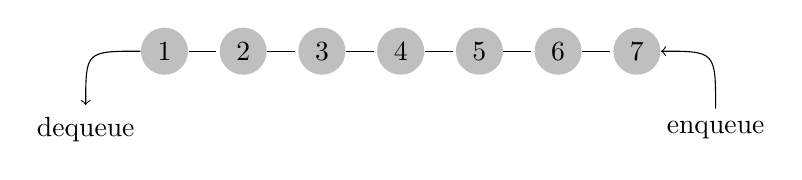
\begin{tikzpicture} [shorten >=1pt,
        vertex/.style={circle,fill=black!25,minimum size=17pt,inner sep=0pt}]
    \foreach \name/\x in {1/1, 2/2, 3/3, 4/4, 5/5, 6/6, 7/7}
        \node[vertex] (G-\name) at (\x,0) {$\name$};
    \foreach \from/\to in {1/2, 2/3, 3/4, 3/4, 4/5, 5/6, 6/7}
        \draw (G-\from) -- (G-\to);
    \node (de) at (0,-1) {dequeue};
    \node (en) at (8, -1) {enqueue};
    \draw [->] (G-1) .. controls (0,0) .. (de); 
    \draw [<-] (G-7) .. controls (8,0) .. (en);
    \end{tikzpicture}
    \caption{队列操作示意图}
\end{figure}

以下是课程之间依赖关系可能构成的图,如果按照这种结构,则序列 \lstinline{[c01, c02, c03, c04, c05, c06]} 就是%
拓扑有序的。

\begin{figure}[H]
    \tikzstyle{house} = [circle, minimum width=8mm, draw=black]
    \tikzstyle{link} = [thick, ->]
    
    \centering
    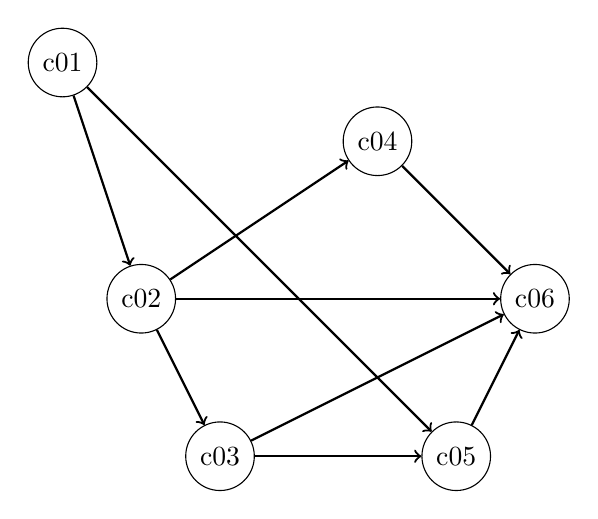
\begin{tikzpicture}
        \node [house] at (-3, 3)  (A) {c01};
        \node [house] at (-2, 0)  (B) {c02};
        \node [house] at (-1, -2) (C) {c03};
        \node [house] at (1, 2)   (D) {c04};
        \node [house] at (2, -2)  (E) {c05};
        \node [house] at (3, 0)   (F) {c06};

        \draw [link ] (A) --  (B);
        \draw [link ] (B) --  (C);
        \draw [link ] (B) --  (D);
        \draw [link ] (C) --  (E);
        \draw [link ] (C) --  (F);
        \draw [link ] (A) --  (E);
        \draw [link ] (B) --  (F);
        \draw [link ] (E) -- (F);
        \draw [link ] (D) --  (F);

    \end{tikzpicture}
    \caption{课程连接模型}
    \label{net}
\end{figure}




\section{逻辑功能}

本项目有以下几个步骤

\begin{enumerate}
    \item 读取输入到程序。
    \item 将课程进行拓扑排序,具体过程是:
    \begin{enumerate}
        \item 初始化一个队列,先将已经规定开课学期的课程入队。
        \item 将入度为0的课程顶点入队。
        \item 对于已经入队的课程,遍历它指向的邻接节点,将他们的入度减一。
        \item 如果减少入度之后入度为0,将它入队。
    \end{enumerate}
    完成后,如果存在还没入队的课程,则说明有循环依赖的存在。
    \item 将队列中的每个课程填入课表,具体流程如下:
    \begin{enumerate}
        \item 如果本学期算上这门课已经超出课时上限,就排到下一个学期。
        \item 如果课程时间大于3课时,先找三节连上的,否则找两节或是一节课的空隙。
        \item 连排时如果2天内已经排了同一门课,就将天数加一。
        \item 如果无法满足要求,则放弃间隔排课的限制,重新从三节联排尝试到一节课的排课。
    \end{enumerate}
    \item 将排好的课程填入字符串并输出。
\end{enumerate}